\chapter{Implementation and Simulation}

\section{Introduction}
This chapter implements and validates the data center design from Chapter 2, translating the spine-leaf topology, VLANs, IP addressing, and redundancy into a working simulation. Challenges and their resolutions are documented below.
\section{Environment}
\subsection{Initial Tool Selection}
\begin{itemize}[nosep]
    \item Planned stack: Huawei eNSP\cite{ensp} + VirtualBox\cite{virtualbox} for servers.
    \item Failure: VirtualBox 5.2.44 crashes on Windows 11; eNSP reached end of life in 2022; Hyper-V conflict.
\end{itemize}
\subsection{Migration to VMware and PNETLab}
\begin{itemize}[nosep]
    \item VMware Workstation Pro 17\cite{vmware} + PNETLab 5.1\cite{pnetlab} + PuTTY\cite{putty} + Linux Debian servers.
    \item Resolved compatibility and multi-NIC requirements.
\end{itemize}
\subsection{Device Image Issues with Huawei CE12800}
\begin{itemize}[nosep]
    \item Unstable boot, 4 ports by default, high RAM (8\,GB+), no MLAG on available image.
\end{itemize}
\subsection{Switch to Arista vEOS}
\hyperref[def:veos]{\underline{Arista vEOS}}: reliable start, 24 ports, 2\,GB RAM, VLANs, trunks, VRRP, and MLAG. All spine and leaf switches were recreated.

\section{Device Configurations}

\subsection{PNETLab interface naming (Arista vEOS)}
Arista vEOS in PNETLab allows only Ethernet interfaces, while the LLD uses different ports. To overcome this challenge, we used the following port mapping in PNETLab:

\begin{table}[htbp]
    \centering
    \small
    \caption{PNETLab (Arista vEOS) to LLD port mapping.}
    \label{tab:pnetlab-port-map}
    \begin{tabular}{|l|l|l|}
        \hline
        \textbf{Switch} & \textbf{LLD interface(s)} & \textbf{PNETLab interface(s)} \\
        \hline
        ToR & \texttt{Ethernet0/0/1}--\texttt{Ethernet0/0/4} & \texttt{Eth1}--\texttt{Eth4} \\
        ToR & \texttt{GigabitEthernet0/0/1}--\texttt{GigabitEthernet0/0/5} & \texttt{Eth5}--\texttt{Eth9} \\
        EoR & \texttt{GigabitEthernet0/0/X} & \texttt{EthX} \\
        \hline
    \end{tabular}
\end{table}

\subsection{Spine switch (EoR-1)}
On EoR-1 we configured: VLANs 110, 120, 130, 210, 220; trunk Port-Channels (Po3--Po10) to all ToR switches; MLAG peer-link Po1 and firewall trunks Po20/Po30; management SVI 10.10.10.208/24 on VLAN~110; MLAG domain \texttt{MLAG-EOR} with peer 10.10.10.209. EoR-2 is configured identically to EoR-1; the only difference is MLAG priority, with EoR-2 operating as the secondary peer. Verification screenshots: Appendix~\ref{app:config-verify}, Figures~\ref{fig:app-eor1-vlans}--\ref{fig:app-eor1-mlag}.

\subsection{Leaf switch (ToR A-1)}
On ToR A-1 we configured: VLANs 110--220; server Port-Channels Po2--Po5 (mgmt/service bonds); uplink Po6 to both EoRs; MLAG peer-link Po1; management 10.10.10.200/24; MLAG domain \texttt{MLAG-TORA} with peer 10.10.10.201. ToR A-2 is configured identically to ToR A-1; the only difference is MLAG priority, with ToR A-2 operating as the secondary peer. Verification: Appendix~\ref{app:config-verify}, Figures~\ref{fig:app-tora1-vlans}--\ref{fig:app-tora1-mlag}.

\subsection{Firewalls (FW-1 and FW-2)}
On FW-1/FW-2 we configured: VLAN sub-interfaces on \texttt{lagg0} (110--220); per-zone IPs (e.g.\ 10.10.10.210 on FW-1); CARP virtual gateways (.254) on all VLANs; zone-based rules (DMZ/Trust separation, default deny). FW-1 master, FW-2 backup. Verification: Appendix~\ref{app:config-verify}, Figures~\ref{fig:app-fw1-vlans}--\ref{fig:app-fw1-rules}.

\subsection{Server (Server 1)}
On Server~1 we configured: \texttt{bond0} 10.10.10.1/24 (mgmt, eth0+eth2); \texttt{bond1} 10.10.20.1/24 (service, eth1+eth3). Servers~2 through~8 are configured identically; only the management and service IP addresses differ according to the LLD. Verification: Appendix~\ref{app:config-verify}, Figure~\ref{fig:app-server1-config}.

\section{Connectivity Testing}

After all devices were configured, ICMP ping tests were executed between Linux servers to validate end-to-end connectivity. Table~\ref{tab:ping-tests} lists every test with its scope (intra/inter cabinet, VLAN, management or service plane, and security zone) and the observed result. Terminal screenshots are provided in Appendix~\ref{app:tests}.

\begin{table}[htbp]
    \centering
    \small
    \caption{Server-to-server ping test results}
    \label{tab:ping-tests}
    \begin{tabular}{|l|l|c|c|c|c|c|}
        \hline
        \textbf{Source} & \textbf{Destination} & \textbf{Cabinet} & \textbf{VLAN} & \textbf{Plane} & \textbf{Zone} & \textbf{Result} \\
        \hline
        Server~1 & Server~2 (10.10.10.2) & A & 110 & Mgmt & Trust & ALLOWED \\
        \hline
        Server~1 & Server~2 (10.10.20.2) & A & 120 & Service & Trust & ALLOWED \\
        \hline
        Server~1 & Server~3 (10.10.20.3) & A--B & 120 & Service & Trust & ALLOWED \\
        \hline
        Server~1 & Server~5 (10.10.30.1) & A--C & 120--130 & Service & Trust & ALLOWED \\
        \hline
        Server~7 & Server~8 (10.20.20.2) & D & 220 & Service & DMZ & ALLOWED \\
        \hline
        Server~1 & Server~7 (10.20.10.1) & A--D & 110--210 & Mgmt & Trust--DMZ & ALLOWED \\
        \hline
        Server~7 & Server~1 (10.10.10.1) & D--A & 210--110 & Mgmt & DMZ--Trust & BLOCKED \\
        \hline
    \end{tabular}
\end{table}

All \texttt{ALLOWED} flows completed successfully, confirming correct VLAN assignment, inter-VLAN routing on the EoR switches, and server bonding. The single \texttt{BLOCKED} test (DMZ--Trust management) validates zone-based firewall policy. Together, the tests cover intra- and inter-cabinet paths, management and service planes, and both intra-zone and inter-zone traffic.

\section{Redundancy \& Failure Testing}

Redundancy was validated by shutting down the active node in each redundant pair and verifying that the standby assumed control. Firewall and EoR pairs were each tested once. At the leaf layer, all four ToR pairs (Cabinets A--D) use the same MLAG active-standby design; the ToR~B test below is documented as representative, because the failover procedure and expected outcome are identical for every cabinet pair.

\subsection{VRRP (CARP) firewall failover test}
\begin{itemize}[nosep]
    \item Stop FW-1; keep pings to CARP gateway addresses.
    \item Observe FW-2 \texttt{MASTER} on all VLANs (Figure~\ref{fig:redund-fw2}).
    \item Result: active-standby firewall failover confirmed.
\end{itemize}
\begin{figure}[htbp]
    \centering
    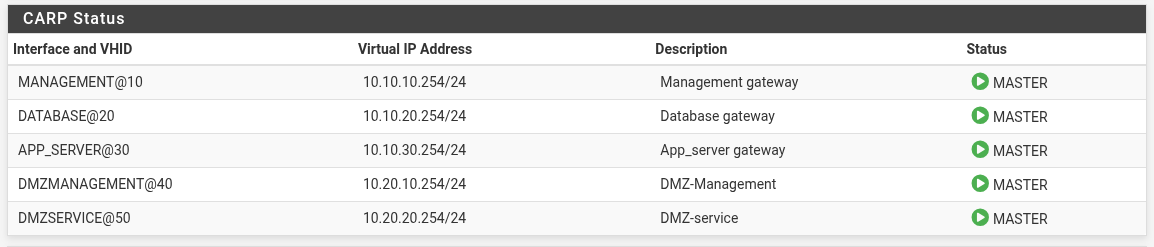
\includegraphics[width=0.72\textwidth,interpolate=false]{figures/redundancy_tests/fw2_after_failover.png}
    \caption{VRRP (CARP) on FW-2 after FW-1 failure.}
    \label{fig:redund-fw2}
\end{figure}

\subsection{EoR MLAG failover test}
\begin{itemize}[nosep]
    \item Shut down EoR-1; run \texttt{show mlag detail} on EoR-2.
    \item Observe \texttt{Failover: True}, cause \texttt{Peer Link Down} (Figure~\ref{fig:redund-eor2}).
    \item Result: backup spine continues forwarding.
\end{itemize}
\begin{figure}[htbp]
    \centering
    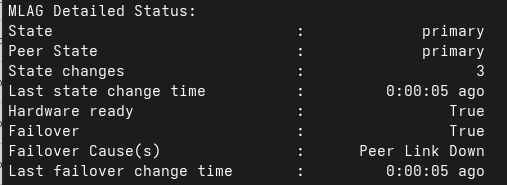
\includegraphics[width=0.65\textwidth,interpolate=false]{figures/redundancy_tests/eor2_after_failover.png}
    \caption{MLAG status on EoR-2 after EoR-1 failure.}
    \label{fig:redund-eor2}
\end{figure}

\subsection{ToR B MLAG failover test}
\begin{itemize}[nosep]
    \item Shut down ToR B-1 with traffic on Cabinet~B servers.
    \item Observe ToR B-2 MLAG primary after peer-link loss (Figure~\ref{fig:redund-torb2}).
    \item Result: leaf active-standby recovery confirmed.
\end{itemize}
\begin{figure}[htbp]
    \centering
    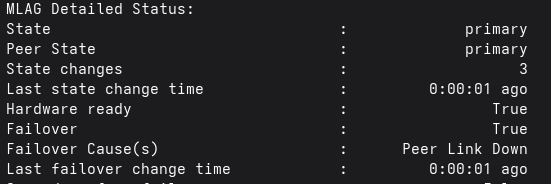
\includegraphics[width=0.65\textwidth,interpolate=false]{figures/redundancy_tests/torb2_after_failover.png}
    \caption{MLAG status on ToR B-2 after ToR B-1 failure.}
    \label{fig:redund-torb2}
\end{figure}

\section{Simulation Environment Status}

% IMAGE: media/image15.png - PNETLab environment screenshot
% \begin{figure}[H]
%     \centering
%     \includegraphics[width=0.9\textwidth]{figures/pnetlab-environment.png}
%     \caption{PNETLab simulation environment showing full topology}
%     \label{fig:pnetlab-env}
% \end{figure}

The final simulation environment runs on:

\begin{itemize}[nosep,itemsep=0pt,topsep=2pt,parsep=0pt,partopsep=0pt]
    \item \textbf{Host:} Windows 11 Pro with VMware Workstation Pro 17
    \item \textbf{PNETLab VM:} 10 vCPUs, 24GB RAM, 100GB storage
    \item \textbf{Total device count:}
    \begin{itemize}[nosep,itemsep=0pt,topsep=0pt,parsep=0pt,partopsep=0pt,leftmargin=1.5em]
        \item 2 spine switches (Arista vEOS)
        \item 8 leaf switches (Arista vEOS)
        \item 2 firewalls (pfSense)
        \item 8 servers (Linux Debian)
    \end{itemize}
    \item \textbf{Resource utilization:} 30\% CPU, 70\% RAM
\end{itemize}

All devices start reliably and maintain stable connections.

\section{Conclusion}
This chapter has presented the complete implementation and validation of the data center design. 
The implemented data center provides a solid foundation for client application deployment, with configuration verification in Appendix~E, connectivity tests in Appendix~D, and LLD tables in Appendix~B.